\chapter{Introduction} \label{introduction}
Large Language Models (LLMs) are transforming various industries by enabling tasks such as automated workflow management using agentic frameworks, information extraction in Natural Language Processing (NLP), and even rudimentary reasoning in some models. In healthcare, LLMs have the potential to assist with clinical note generation, medical summarization, diagnosis support, and personalized patient care.

Despite these capabilities, LLMs suffer from a well-documented issue known as hallucinations, where they generate seemingly coherent but incorrect information. This has potentially disastrous complications in high-stakes domains such as medicine, law, and cybersecurity, where misinformation can lead to severe consequences.

To address this, Retrieval-Augmented Generation (RAG) is commonly used to supplement LLMs with external knowledge sources, improving factual accuracy by providing the LLM with context to generate from. While RAG enhances LLM performance, it also introduces new security risks. In particular, threat actors can exploit prompt injection attacks, in a similar fashion to LLMs, to manipulate retrieval outputs or extract sensitive data, which poses a significant privacy threat—especially in healthcare, where patient confidentiality is critical.

In this project, we an Agent-based synthetic document generation framework designed to mitigate these risks. By separating the RAG database from the externally facing LLM, we ensure the sensitive records are not directly exposed to the model. Instead, they undergo a controlled synthesis process. Only the necessary information is extracted from the retrieved knowledge, and any appearance of sensitive information such as names and ages are replaced with placeholders before being passed to the external LLM. This reduces the likelihood of data leakage while preserving response accuracy.

In chapter \ref{introduction} we provide a brief description of a RAG system as well as briefly discuss applications of LLMs with RAG in healthcare.

\section{Background}

\subsection{Retrieval-Augmented Generation (RAG)}
% TODO: Add a section about RAG here
While LLMs are often trained on large datasets which, at times, provide the illusion that they have knowledge on many different fields, LLMs are still, first and foremost, text prediction engines used for Natural Language Processing (NLP) tasks.

This results in the following consequence: When an LLM encounters a query about information outside its training set, it will attempt to generate a response that is gramatically coherent, but potentially unsound response, a phenomenon known as hallucination. Depending on the applications, hallucinations can range from minor inaccuracies to critical failures, such as generating false legal cases \autocite{Bohannon_2024} or misdiagnosing medical conditions.

Retrieval-augmented generation (RAG), first introduced by \autocite{lewis2021retrievalaugmentedgenerationknowledgeintensivenlp}, was developed to mitigate hallucinations by integrating an external knowledge base into the LLM's generation pipeline. This grounds the LLMs respone using the retrieved knowledge, preventing speculative responses from the LLM when faced with tokens outside its training set.

\begin{figure}
	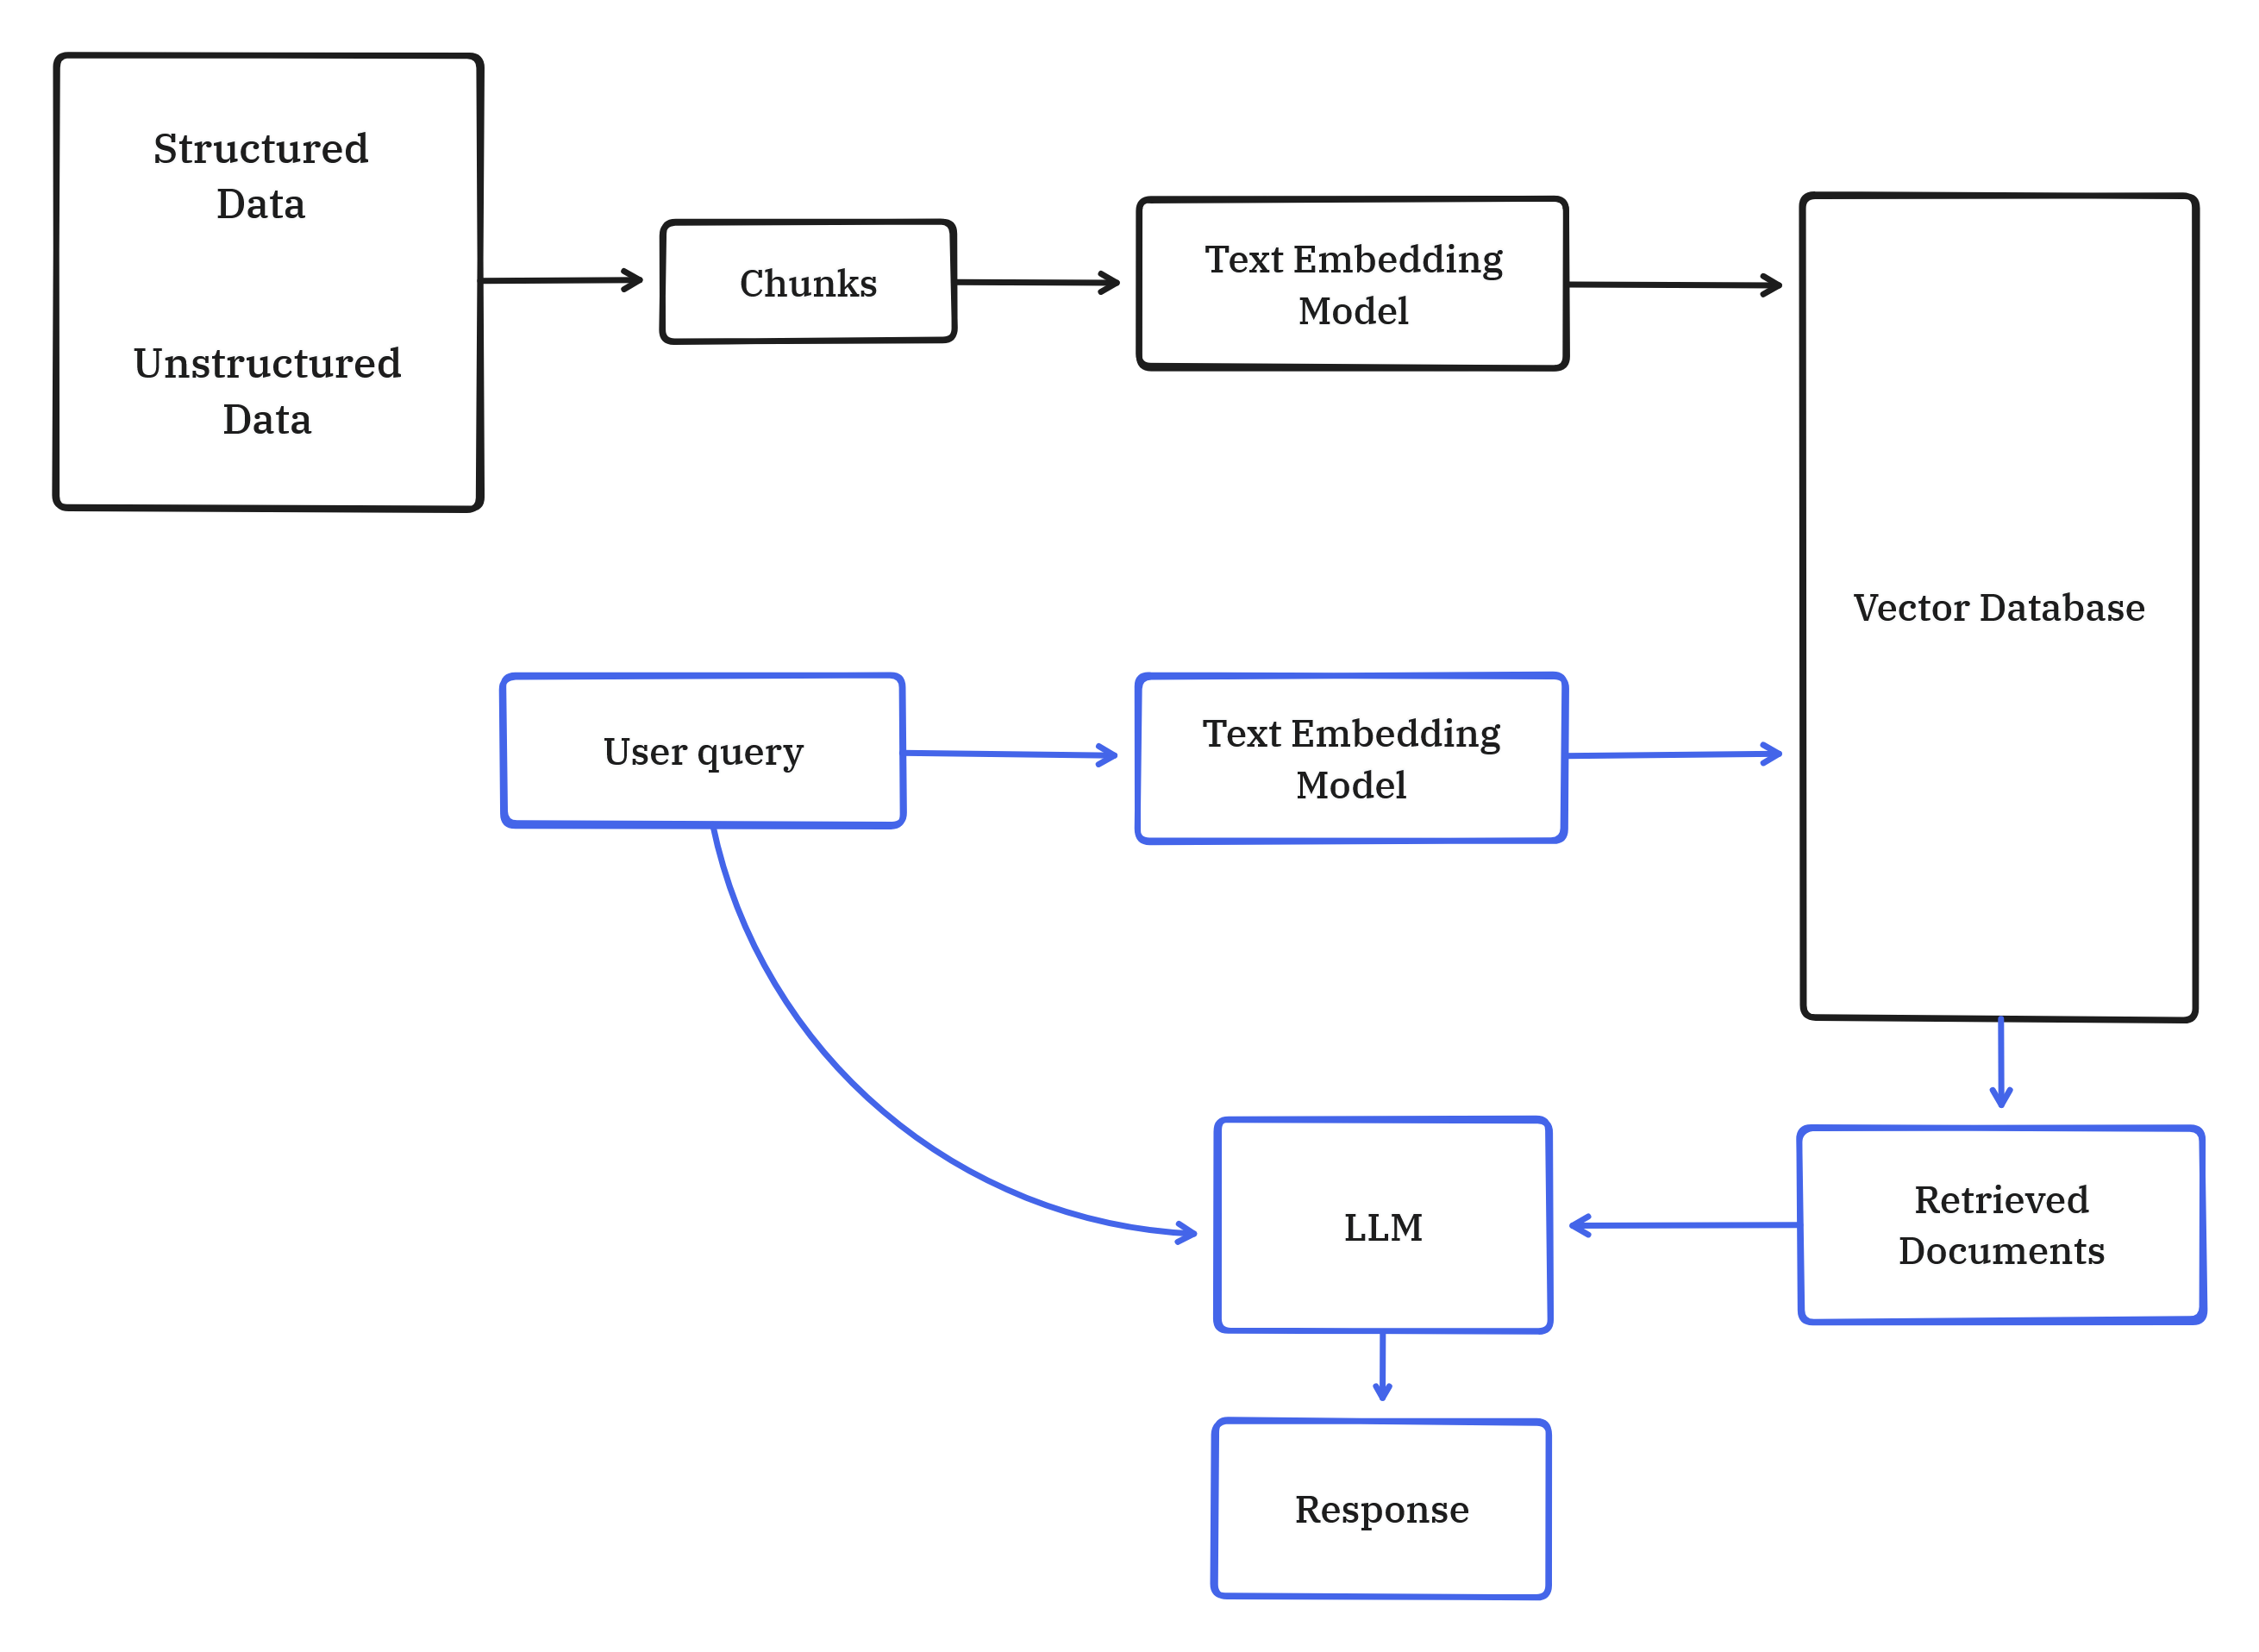
\includegraphics[width=\textwidth]{Conventional RAG example.png}
	\caption{Example of a Conventional RAG system}
	\centering
	\label{fig:RAGexample}
\end{figure}

RAG operates by retrieving relevant documents from an unstructured or structured vector database and providing them as context for response generation. To facilitate retrieval, documents are converted into vector representations using a text embedding model, which captures the semantic relations in text. When a query is presented to an LLM with a RAG system, the query undergoes the same text embedding process. The vectorized query is compared with the document vectors present in the database and those that have the highest similarity are returned to the LLM.

Through RAG, an LLM becomes able to generate highly accurate, domain-specific information rather than rely on its pre-trained knowledge, allowing for flexible applications in various fields.

One application of RAG in healthcare is in diagnostic assistance, where LLMs match patient symptoms with medical knowledge retrieved from external sources. This enables more informed diagnoses while reducing the cognitive load on physicians. Furthermore, LLMs may be able to detect subtle symptom correlations that clinicians might overlook, improving early disease detection \autocite{jin2024healthllmpersonalizedretrievalaugmenteddisease}.


While RAG brings many benefits, it comes with its own caveats. RAG systems remain susceptible to prompt attacks much like LLMs are. They can also become poisoned, where the RAG corpus becomes corrupted through the insertion of adversarial attack passages.

In chapter \ref{literature} we discuss more about the vulnerabilities that RAG systems have.

\subsection{LLMs in Healthcare}

For Singapore in particular, LLMs have seen increased usage in healthcare. In 2013, Singapore's National University Health System (NUHS) launched its very own LLM, Russell-GPT, that was used for summarizing patient clinical notes, automating referral letter generation, as well as predict the healthcare journeys for patients \autocite{NUHS_2023}.

Singapore has also developed an LLM capable of understanding the local english dialect, Singlish, which has deployed in various settings, including clinics and emergency response systems, where it is used in transcribing emergency calls \autocite{Chia_2024}.

These developments showcase the growing reliance on LLMs in Singapore's healthcare ecosystem, highlighting their potential to improve the efficiency of its healthcare system. However, as LLMs become increasingly integrated into critical systems, it is essential to address the risks of their use - particularly when augmented with enhancements like RAG. RAG-powered LLMs remain vulnerable to adversarial attacks, risking the exposure of sensitive medical information. As such, ensuring that the security and privacy of LLM-based solutions remains a priority as they continue to evolve.
